\section{N2}
\subsection*{Material ID: mp-bmgle}
\textbf{Constante Dieléctrica ($\epsilon_{total}$):} 1.40 \\[0.5em]
\begin{table}[h!]
\centering
\begin{tabular}{lcc}
\toprule
\textbf{Métrica} & \textbf{Lámina (Plate)} & \textbf{Cilindros (Rod)} \\
\midrule
Bandgaps ($a/\lambda$) & Ninguno & Ninguno \\
Resonancias & 36 & 36 \\
\bottomrule
\end{tabular}
\end{table}
\begin{figure}[H]
\centering
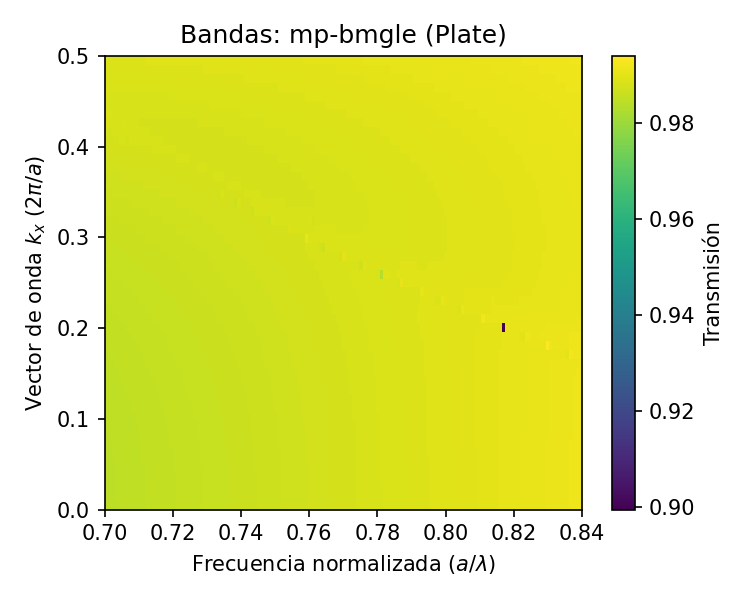
\includegraphics[width=0.48\textwidth]{figures/mp-bmgle_plate.png}
\hfill
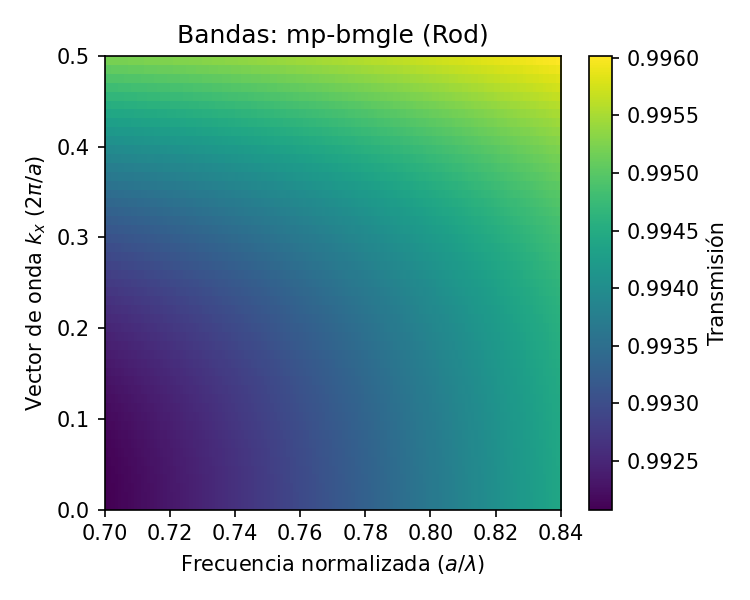
\includegraphics[width=0.48\textwidth]{figures/mp-bmgle_rod.png}
\caption{Estructuras de bandas fotónicas para mp-bmgle. Izquierda: Lámina. Derecha: Cilindros.}
\end{figure}
\vspace{1em}
\hrule
\vspace{1em}
\subsection*{Material ID: mp-cewog}
\textbf{Constante Dieléctrica ($\epsilon_{total}$):} 5.01 \\[0.5em]
\begin{table}[h!]
\centering
\begin{tabular}{lcc}
\toprule
\textbf{Métrica} & \textbf{Lámina (Plate)} & \textbf{Cilindros (Rod)} \\
\midrule
Bandgaps ($a/\lambda$) & Ninguno & Ninguno \\
Resonancias & 36 & 36 \\
\bottomrule
\end{tabular}
\end{table}
\begin{figure}[H]
\centering
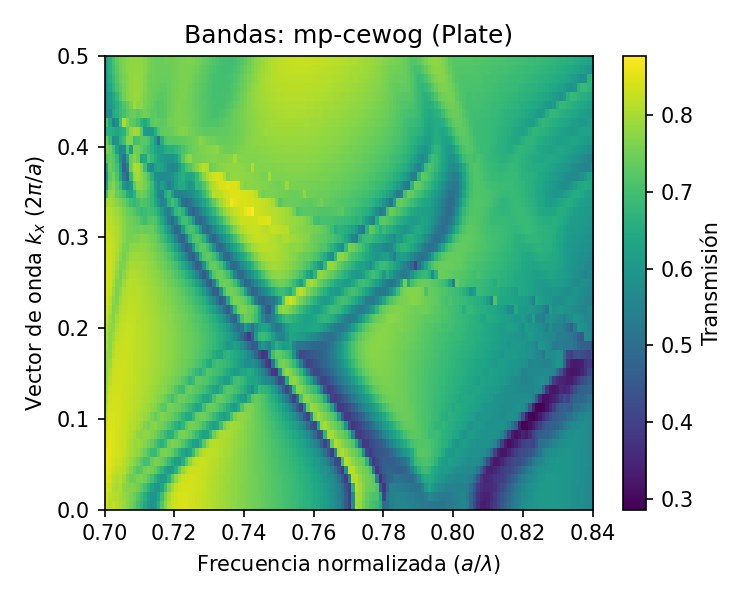
\includegraphics[width=0.48\textwidth]{figures/mp-cewog_plate.png}
\hfill
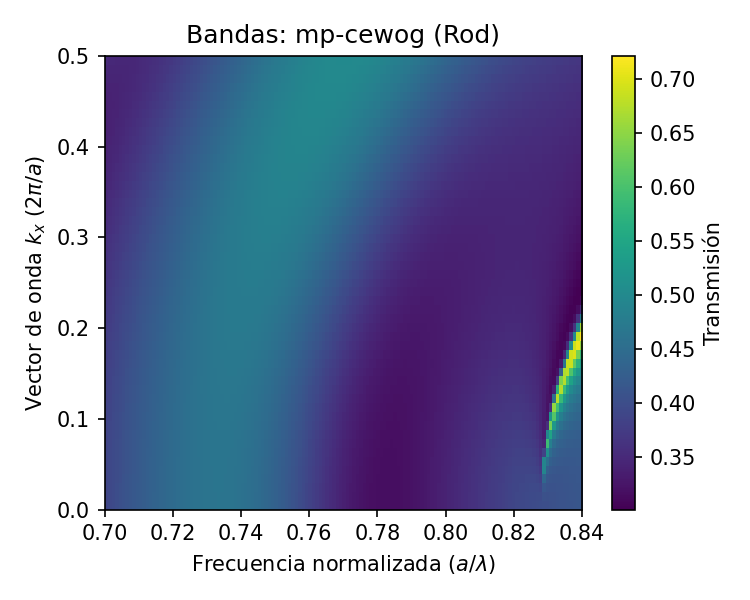
\includegraphics[width=0.48\textwidth]{figures/mp-cewog_rod.png}
\caption{Estructuras de bandas fotónicas para mp-cewog. Izquierda: Lámina. Derecha: Cilindros.}
\end{figure}
\vspace{1em}
\hrule
\vspace{1em}
\subsection*{Material ID: mp-fy}
\textbf{Constante Dieléctrica ($\epsilon_{total}$):} 1.53 \\[0.5em]
\begin{table}[h!]
\centering
\begin{tabular}{lcc}
\toprule
\textbf{Métrica} & \textbf{Lámina (Plate)} & \textbf{Cilindros (Rod)} \\
\midrule
Bandgaps ($a/\lambda$) & Ninguno & Ninguno \\
Resonancias & 36 & 36 \\
\bottomrule
\end{tabular}
\end{table}
\begin{figure}[H]
\centering
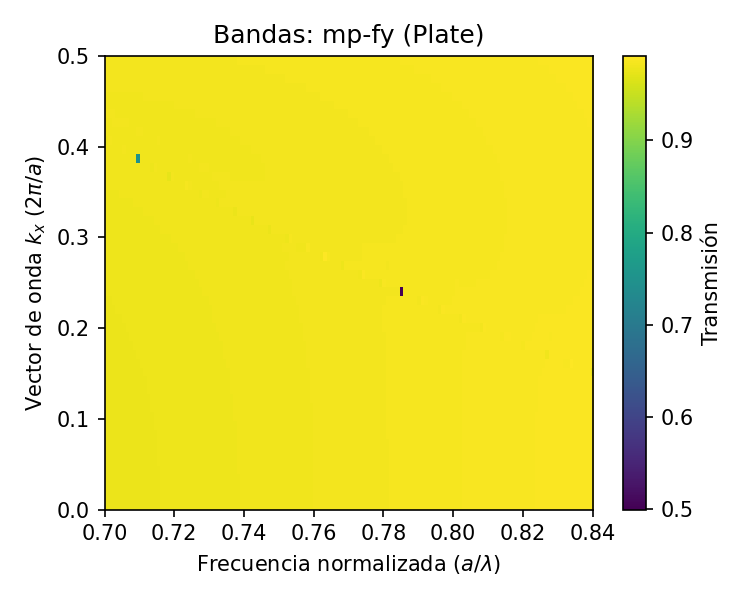
\includegraphics[width=0.48\textwidth]{figures/mp-fy_plate.png}
\hfill
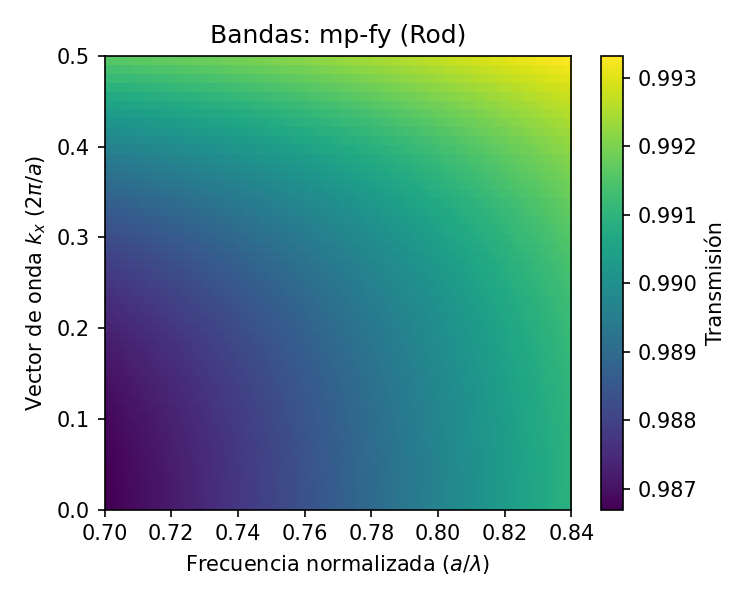
\includegraphics[width=0.48\textwidth]{figures/mp-fy_rod.png}
\caption{Estructuras de bandas fotónicas para mp-fy. Izquierda: Lámina. Derecha: Cilindros.}
\end{figure}
\vspace{1em}
\hrule
\vspace{1em}
\subsection*{Material ID: mp-rxn}
\textbf{Constante Dieléctrica ($\epsilon_{total}$):} 1.41 \\[0.5em]
\begin{table}[h!]
\centering
\begin{tabular}{lcc}
\toprule
\textbf{Métrica} & \textbf{Lámina (Plate)} & \textbf{Cilindros (Rod)} \\
\midrule
Bandgaps ($a/\lambda$) & Ninguno & Ninguno \\
Resonancias & 36 & 36 \\
\bottomrule
\end{tabular}
\end{table}
\begin{figure}[H]
\centering
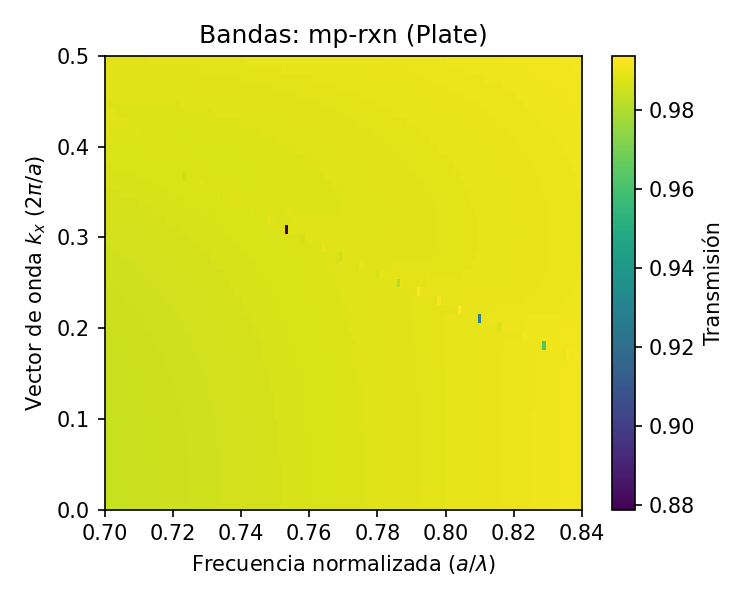
\includegraphics[width=0.48\textwidth]{figures/mp-rxn_plate.png}
\hfill
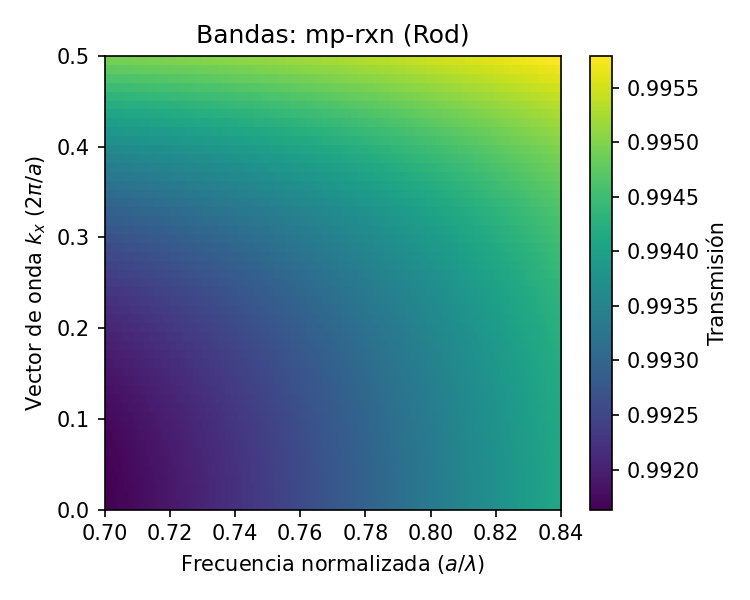
\includegraphics[width=0.48\textwidth]{figures/mp-rxn_rod.png}
\caption{Estructuras de bandas fotónicas para mp-rxn. Izquierda: Lámina. Derecha: Cilindros.}
\end{figure}
\vspace{1em}
\hrule
\vspace{1em}
\clearpage